\section{Experiments} \label{sec:experiment}

We measure the performance of the HLS based BFS 
accelerator on Alpha Data ADM-7v3 and KU115 using a set of 
representative graphs and compare them to both a 
baseline design and previous handcrafted BFS accelerators. 
The baseline design refers to a design with HLS pragmas 
added to the native C based level synchronous BFS implementation. 
Then we briefly evaluate the design optimization 
methods including pipelining, redundancy removal, 
caching and data path duplication 
proposed in this work. Based on the design on ADM-7v3, 
we further ported the design 
to KU115 on Nimbix Cloud and explored the portability of the 
BFS accelerator. 



\subsection{Experiment Setup}
The graph benchmark used in this work includes three real-world graphs and 
two synthetic graphs generated using R-MAT model \cite{chakrabarti2004rmat} 
as listed in Table \ref{tab:graph}. The real-world graphs are from social network 

\cite{snapnets} while the R-MAT graphs are generated 

using the Graph 500 benchmark parameters ($A=0.59, B=0.19, C=0.19$). To make the 

presentation easier, the five benchmark graphs are shorted as Youtube, 

LJ, Pokec, R-MAT\uppercase\expandafter{\romannumeral1}, 

R-MAT\uppercase\expandafter{\romannumeral2} respectively. We refer 

to an R-MAT graph with scale $S$ ($2^{S}$ nodes) and edge factor $E$ ($E\times 2^{S}$). 

In order to avoid trivial search, we only choose vertices from the largest 

connected component as the BFS starting point.



\begin{table}

    \centering

  \vspace{-0.3em}

  \caption{Graph Benchmark}

  \label{tab:graph}

  \vspace{-0.3em}

  \begin{tabular}{cccc}

    \toprule

      Name & \# of vertex & \# of edge & Type \\

    \midrule

      Youtube & 1157828 & 2987624 & Undirectional \\

      LJ & 4847571 & 68993773 & Directional \\

      Pokec & 1632804 & 30622564 & Directional \\

      R-MAT\uppercase\expandafter{\romannumeral1} & 524288 & 16777216 & Directional \\

      R-MAT\uppercase\expandafter{\romannumeral2} & 2097152 & 67108864 & Directional \\

  \bottomrule

\end{tabular}

\vspace{-1em}

\end{table}



\subsection{Performance comparison}

We use the million traverse per second (MTEPS) as 

the performance metric. The performance of the proposed BFS 

accelerator on the graph benchmark is 

presented in Table \ref{tab:performance-summary}. 

The implementation on ADM-7v3 achieves up to 

82.16 MTEPS on the R-MAT\uppercase\expandafter{\romannumeral1} graph. 

When compared to a baseline HLS based 

BFS accelerator, the proposed design shows 24.7X to 77.5X performance 

speedup on the benchmark. 

With the comparison, it is clear that straightforward HLS optimizations 

are far from sufficient and dedicated high level optimizations are critical to 

the performance of the resulting BFS accelerator.

\begin{table}

  \vspace{-0.3em}

    \centering

  \caption{Performance summary}

  \vspace{-0.3em}

  \label{tab:performance-summary}

  \begin{tabular}{cccccc}

    \toprule

      Benchmark & Youtube & LJ & Pokec & RMAT\uppercase\expandafter{\romannumeral1} & RMAT\uppercase\expandafter{\romannumeral2} \\

    \midrule

      MTEPS & 14.35 & 28.05 & 36.94 & 82.16 & 32.67 \\

      Speedup & 77.50 & 36.82 & 38.83 & 62.18 & 24.70 \\

  \bottomrule

\end{tabular}

\vspace{-1em}

\end{table}



We also compare this work to a set of existing BFS accelerators on FPGAs. 

As the platforms and graph benchmarks used in these work are mostly different and it is 

difficult to make a complete fair end-to-end comparison. Here just use R-MAT graph for the comparison. 

We provide two implementations on Alpha-Data ADM-7v3 and KU115 respectively. A rough comparison result is listed 

in Table \ref{tab:compare}. The best HLS based BFS implementation on KU115 is 

getting close to that in \cite{zhang2017boosting}, though the peak memory bandwidth 

is relatively higher. When compared to design on high-end 

FPGA computing system such as Convey HC-2 with highly optimized memory sub systems, 

the performance is still much lower. 



Since different FPGAs may have diverse memory bandwidth, we also measure the 

per bandwidth BFS performance i.e. MTEPS/GB. According to the experiments, we 

can see that the HLS based BFS accelerator on Alpha-Data achieves higher 

MTEPS/GB. The comparison shows that the memory bandwidth on KU115 is not 

fully explored. This is mainly caused by the fact that only 16 global memory 

ports are allowed to be implemented in the SDAccel design and 

limited parallel data paths can be instantiated on the FPGAs as 

mentioned in previous section. We believe the performance of the 

proposed design can be further improved given more parallel data paths.



\begin{table}

  \vspace{-0.3em}

  \caption{FPGA based BFS accelerator comparison}

  \label{tab:compare}

    \setlength{\tabcolsep}{4pt} % Default value: 6pt

    %\renewcommand{\arraystretch}{1.5} % Default value: 1

  \vspace{-0.3em}

  \begin{tabular}{cccccc}

    \toprule

      Work & Platform & Graph & MTEPS & BW(GB/s) & MTEPS/GB \\

    \midrule

      \cite{betkaoui2012reconfigurable} & Convey HC-2 & R-MAT & 1600 & 80  & 20 \\

      \cite{attia2014cygraph} & Convey HC-2 & R-MAT    & 1900 & 80  & 23.8 \\

      \cite{zhang2017boosting} & Micro-AC510       & R-MAT  & 166.2  & 60  & 2.8 \\

      this work & ADM-7v3 & R-MAT & 57.41 & 10.8 & 5.3 \\

	  this work & KU115 & R-MAT & 120.84 & 76.8 & 1.57\\

  \bottomrule

\end{tabular}

\vspace{-1em}

\end{table}



\subsection{Design Configuration and Resource Overhead}

With the software emulation based tuning, 

we can decide the design configurations rapidly. The graph specific configuration 

of the BFS accelerator targeting ADM-7v3 is summarized in 

Table \ref{tab:parameter-setup}. The hash tables for LJ and R-MATII 

as highlighted in the table are shrunk to fit for the on-chip memory constraints. 

Note that the \textit{depth} read and write cache 

are set to be the same and the cache size in the table refers to the capacity of 

one cache size.



\begin{table}

  \vspace{-0.3em}

  \caption{Memory optimization parameter setup on ADM-7v3}

  \label{tab:parameter-setup}

  %\setlength{\tabcolsep}{4pt} % Default value: 6pt

  %\renewcommand{\arraystretch}{1.5} % Default value: 1

    \centering

  \vspace{-0.3em}

  \begin{tabular}{ccccccc}

    \toprule

      Benchmark & Hash Table & Cache Size & Prefetch Buffer \\

    \midrule

      Youtube  & 256K  & 16K $\times$ 64B & 64B \\

      LJ       & \textbf{512K} & 32K $\times$ 64B & 64B \\

      Pokec    & 1024K & 16K $\times$ 64B & 64B \\

      R-MATI   & 512K  & 8K $\times$  64B & 64B \\

      R-MATII  & \textbf{512K} & 32K $\times$ 64B & 64B \\

  \bottomrule

\end{tabular}

\vspace{-1em}

\end{table}



The corresponding FPGA resource consumption is 

presented in Table \ref{tab:mem-resource}. 

FF and LUT consumption do not change much with the different 

design configurations and they take up only a small portion 

of the total FPGA resources. Block RAMs turns out to be the major 

resource bottleneck, and it leads to the adoption of sub optimal 

design configurations.



\begin{table}

  \vspace{-0.5em}

  \caption{FPGA resource consumption on ADM-7v3}

  \label{tab:mem-resource}

  \vspace{-0.3em}

  %\setlength{\tabcolsep}{4pt} % Default value: 6pt

  %\renewcommand{\arraystretch}{1.5} % Default value: 1

    \centering

  \begin{tabular}{ccccccc}

    \toprule

      Config. & FF & \% & LUT & \% & RAMB18K & \% \\

    \midrule

      Youtube  & 65244 & 7 & 108810 & 25 & 1515  & 51 \\

      LJ       & 65266 & 7 & 108829 & 25 & 2784  & 94 \\

      Pokec    & 65262 & 7 & 108812 & 25 & 2155 & 73 \\

      R-MATI   & 65244 & 7 & 108808 & 25 & 1217 & 41 \\

      R-MATII  & 65266 & 7 & 108829 & 25 & 2784 & 94 \\

  \bottomrule

\end{tabular}

\vspace{-1em}

\end{table}



\subsection{Optimization evaluation}

In this section, we evaluate the 

performance of the BFS accelerators with the different optimizations. 

Basically we start from the baseline design and 

add the optimizations including pipelining, hash redundancy removal, 

prefetching, caching and data path duplication in order. The performance improvement 

can be found in Figure \ref{fig:opt-performance}. 

In general, the performance of the BFS accelerator improves 

significantly when more optimization techniques are applied. Particularly,

pipelining and data path duplication enhance the performance most. 

The performance improvement brought by the hash table based filtering 

seems to be trivial, but it actually boosts the performance by over 20\% on average. 

In addition, it also affects the cache efficiency as observed in Section \ref{sec:observation}

and is thus critical to the overall accelerator performance.



\begin{figure}

\center{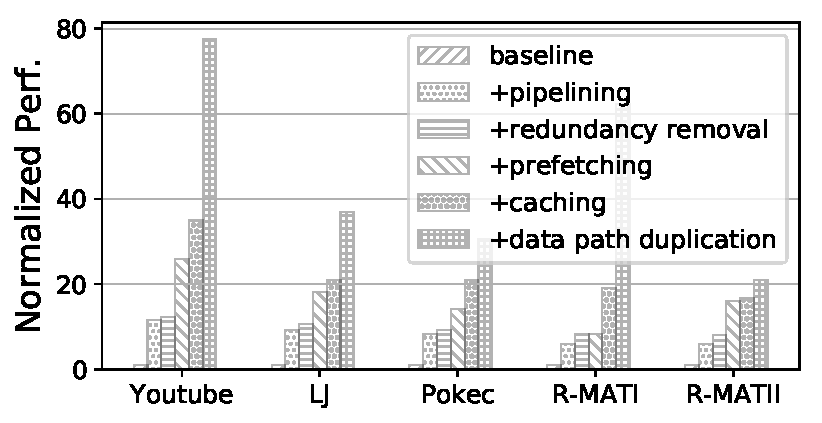
\includegraphics[width=0.85\linewidth]{opt-performance}}

    \caption{BFS accelerator optimization technique evaluation. The performance on 

    all the graphs improves when more optimizations including pipelining, 

    redundancy removal, prefetching, caching, and data path duplication are 

    gradually applied to the design.}

\label{fig:opt-performance}

\vspace{-1em}

\end{figure}



There is only one memory bank available in ADM-7v3, so we 

evaluate the memory bank-aware data layout strategy by porting the design to KU115.

Without the bank-aware layout optimization, porting the design from ADM-7v3 to 

KU115 achieves less performance improvement despite the much larger memory 

bandwidth on KU115. When the optimization is applied, the multiple-bank memory 

on KU115 can be utilized. The performance of the BFS accelerator on KU115 improves 

significantly as shown in Table \ref{tab:porting-summary} especially for the 

graphs with more edges. This experiment also 

demonstrated the portability of the proposed HLS based BFS accelerator.

\begin{table}

	\vspace{-0.5em}

    \centering

	\caption{Memory-bank aware data layout optimization influence on the BFS accelerator performance (MTEPS)}

  \label{tab:porting-summary}

  \vspace{-0.3em}

  \begin{tabular}{cccccc}

    \toprule

	Benchmark & Youtube & LJ & Pokec & RMAT\uppercase\expandafter{\romannumeral1} & RMAT\uppercase\expandafter{\romannumeral2} \\

    \midrule

	ADM-7v3 & 14.35 & 28.05 & 36.94 & 82.16 & 32.67 \\

	KU115 with bank opt. & 18.69 & 61.49 & 68.04 & 122.48 & 119.2 \\

	KU115 no bank opt. & 14.15 & 41.74 & 40.82 & 85.18 & 63.31\\

  \bottomrule

\end{tabular}

\vspace{-1em}

\end{table}





\section{Insights and Conclusions} \label{sec:conclusion}

\subsection{Insights}

From this study, we have obtained a few insights on HLS based graph processing.

1) The high level design tools are able to produce competitive

hardware implementations for irregular graph algorithms. Given more efforts, we can 

create a library of HLS based graph processing algorithms in which each algorithm 

can be highly customized for higher performance. In this case, 

this can be a competitive alternative to the RTL based graph processing framework 

which also sacrifices the performance for the design productivity.

2) Random memory access and short sequential memory access are frequent memory access patterns.

They can be optimized using the common wisdom such as caching and prefetching. However, 

building these logic using the HLS is error-prone and inefficient. If they are integrated into 

the memory access port and allows the designers to decide when it can be utilized. 

The HLS design tools can be beneficial to more applications with irregular memory access.

3) Optimizing the HLS design for higher performance is non-trivial. It is not

so much friendly to software programmers as expected. Hardware design

experiences are important for optimizing the HLS based design.



\subsection{Conclusions}

Handcrafted HDL based BFS accelerators usually suffer 

high portability and maintenance cost 

as well as ease of use problem despite the relatively 

good performance. HLS based BFS accelerator can greatly 

alleviate these problems, but it is 

difficult to achieve satisfactory performance due to 

the inherent irregular memory access and 

complex nested loop structure. In this work, we developed 

a series of HLS based optimizations such as redundancy removal, 

prefetching, caching and data path duplication. 

With the optimizations, BFS performance can be greatly improved. 

According to the experiments on 

a representative graph benchmark, the resulting HLS based BFS accelerator 

achieves up to 70X speedup compared to a baseline HLS design. 

When compared to the existing HDL based BFS accelerators on 

similar FPGA cards, the proposed HLS based BFS accelerator on KU115 

gets over 70\% of the MTEPS while it still preserves the 

software-like features including portability and ease of use 

and maintenance.  
